\documentclass[]{article}
\usepackage{amsmath}
\usepackage{graphicx}
\usepackage{subcaption}
\usepackage{geometry}
\geometry{
  a4paper,
  total={6in,9.5in}
}

%opening
\title{A Flexible and Efficient Modeling Strategy for Trend Analysis of North American Bird Count Data}
\author{T. D. Meehan, N. L. Michel, H. Rue}

\begin{document}
\maketitle

\section{Motivation}
Volunteers with the Audubon Christmas Bird Count (CBC, Soykan et al. 2016) have been counting wintering birds across North America every year for the last 118 years. Population trends derived from CBC data, along with those derived from other large-scaled monitoring programs like the North American Breeding Bird Survey (BBS, Sauer and Link 2011), are important pieces of information for understanding the conservation needs of North American bird species (Partners in Flight 2016).

The current standard approach for generating trends from CBC data (Link et al. 2006, Soykan et al. 2016) is based on methods originally developed for BBS data (Link and Sauer 2002, Sauer and Link 2011). The general approach is to (\textit{i}) assign counts in Canada and the US to roughly 150 spatial strata, which are intersections of US states, Canadian provinces, and Bird Conservation Regions (BCR, North American Bird Conservation Initiative, Figure 1A). Then, treating each stratum as independent, (\textit{ii}) use a non-linear function to remove the effect of observer effort on counts, and (\textit{iii}) model the residual as a function of count circle identifier, stratum, and year. Next, (\textit{iv}) model parameters are used to derive a relative abundance index per stratum and year, and (\textit{v}) those indices are used to compute percent change per stratum across different time intervals.

The pros of the current CBC approach are as follows. (\textit{i}) By pooling count circles per stratum, this approach deals with the issue of count locations haphazardly becoming active or inactive over the time series. (\textit{ii}) By pooling per stratum, a large enough sample of counts is attained to generate a reasonably robust count-effort correction function. (\textit{iii}) The approach produces a relative abundance index per year and stratum, which can be summed across larger strata, such as states, provinces, or BCRs, and used to calculate temporal trends at larger spatial scales. 

\begin{figure}[t]
  \centering
  \begin{subfigure}[t]{0.95\textwidth}
    \centering
    \includegraphics[width=\textwidth]{different_strata} 
  \end{subfigure}
  \caption{Spatial strata from the standard CBC approach (Soykan et al. 2016, A) and grid cells used for the current analysis, which are similar to those used by Bled et al. (2013, B).}
\end{figure}

The cons of the current approach are as follows. (\textit{i}) It is computationally intensive, especially for wide-ranging species such as the American Robin, as it uses Markov chain Monte Carlo (MCMC) to estimate model parameters for relative abundance, and then processes large MCMC chains to scale relative abundance to larger aggregate units and generate trend estimates. (\textit{ii}) While trends can be scaled up to larger aerial units, they cannot be scaled down to smaller ones. The analytical strata is the finest level of resolution, which limits the extent to which trends can be attributed to specific factors occurring at finer spatial scales (Thogmartin et al. 2004, Bled et al. 2013). (\textit{iii}) It does not take full account or full advantage of spatial relationships in counts. Modeling this structure would facilitate borrowing information across spatial boundaries, allowing more robust trend estimates in places where there is a shortage of data (Thogmartin et al. 2004, Bled et al. 2013). Indeed, borrowing information would allow trends to be estimated at spatial scales that are finer than the spatial strata currently used.

\begin{figure}[t]
  \centering
    \begin{subfigure}[t]{0.93\textwidth}
    \centering
    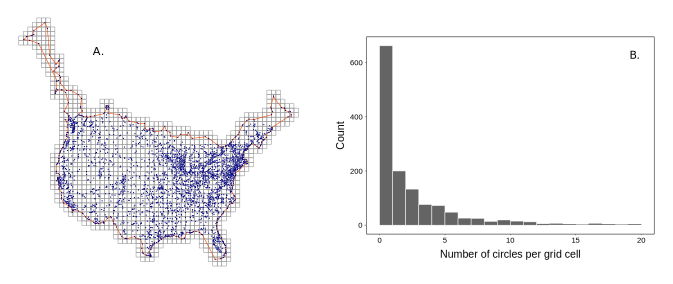
\includegraphics[width=\textwidth]{gridding} 
  \end{subfigure}
    \caption{(A) CBC locations (blue points), along with the non-convex hull (red), and grid cells (gray) used for this analysis of American Robin data. (B) The number of CBC locations per grid cell.}
\end{figure}

Work by Thogmartin et al. (2004), Bled et al. (2013), and Smith et al. (2015) offered spatially-explicit variations of the standard trend analysis approach. These works were focused on analysis of BBS data, but their approaches are easily related to analysis of CBC data. Their approaches contrasted with the standard approach, described above, in the following ways. (\textit{i}) Instead of using the standard strata described above, Thogmartin et al. (2004) assigned count sites to irregular polygons, created by tessellation of BBS route locations.  Bled et al. (2013) assigned routes to cells on a regular grid, with one-degree latitude and longitude spacing (similar to Figure 1B). (\textit{ii}) All three studies utilized a spatially-structured (intrinsic conditional autoregressive model, ICAR, Besag et al. 1991) intercepts for relative abundance per polygon or grid cell. (\textit{iii}) Thogmartin et al. (2006) utilized a fixed effect of time per BBS route, but that effect did not incorporate spatial structure. (\textit{iv}) Bled et al. (2013) and Smith et al. (2015) did not include a fixed effect of time. Instead, they estimated relative abundances per year, and then trends were generated as a derived parameter during MCMC simulations.

\begin{figure}[t]
  \centering
  \begin{subfigure}[t]{0.99\textwidth}
    \centering
    \includegraphics[width=\textwidth]{trend_and_index} 
  \end{subfigure}
  \caption{American Robin trends (A), along with the width of the 95\% credible interval (B) per grid cell. Trends are $\tau$ values that are exponentiated and converted to a percent. (C) The cells from (A) that are significantly different from zero. (D) The abundance index per grid cell, $\alpha$, which is the exponentiated sum of the global intercept, AR1, and ICAR terms.}
\end{figure}

Here, we present a different approach for calculating temporal trends in relative abundance, one that takes advantage of both spatial structure in CBC data. This approach borrows components from previous ones, incorporates new components that prioritize robust trend estimation at finer spatial scales, and employs a relatively simple and computationally efficient process. Similar to Bled et al. (2013), we assigned CBC count sites to cells on a uniform grid that covered North America. Like Thogmartin et al. (2004), temporal trends were explicit components of the model. In contrast to previous work, effort and year effects were modeled as random slopes with spatial structure, following a spatially varying coefficient (SVC) approach (Congdon 2014). Finally, unlike prior studies using MCMC, we used integrated nested Laplace approximation (INLA) to estimate Bayesian posteriors for model parameters, which led to a considerable decrease in computing time.

\section{Model}
We modeled Christmas Bird Counts, $y_{i,k,t}$ for grid cell \textit{i} encompassing count circle \textit{k} during year \textit{t}, as an overdispersed Poisson random variable (Link and Sauer 2002, Link et al. 2006). Expected values for counts per grid cell, $\lambda_{i,t}$, were assumed to be a function of spatially-structured grid-cell, count-effort, and year effects. The linear predictor for $\lambda_{i,t}$ took the form

$$\text{log}(\lambda_{i,t}) = \alpha _{i} + \epsilon_{i} \text{log}(E_{i,k,t}) + \tau_{i}T_{i,k,t} + \omega_{i,k,t}.$$

$\alpha_i$ was a cell-specific relative abundance term that comprised the sum of three components, $\alpha_i = \alpha_0 + \psi_i + \upsilon_i$. The first component, $\alpha_0$, was a global intercept averaged over all grid cells and years. The second component, $\psi_i$, was an exchangeable random effect per cell, modeling deviations from the global intercept as unstructured and normally distributed. The third component $\upsilon_i$ was a spatially-structured random effect per cell, modeling deviations from the global intercept with ICAR structure, where values came from a normal distribution, with a conditional mean related to the average of adjacent cells, and with conditional variance proportional to the variance across adjacent cells and inversely proportional to the number of adjacent cells. Spatial structure was incorporated into $\alpha_i$ to allow for information about relative abundance to be shared across neighboring cells.

\begin{figure}[t]
  \centering
  \begin{subfigure}[t]{0.99\textwidth}
    \centering
    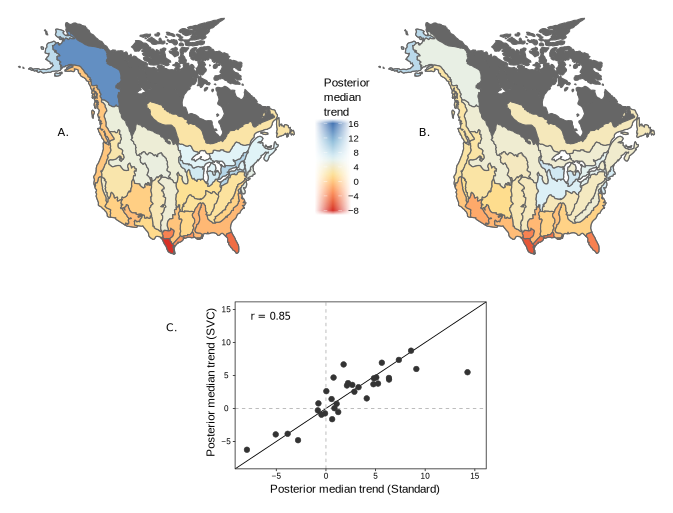
\includegraphics[width=\textwidth]{bcr_comparison} 
  \end{subfigure}
  \caption{Map of American Robin posterior median trends per BCR, produced using the standard analysis approach (A) and the one demonstrated here (B). (C) Bivariate plot of the trends mapped in (A) and (B), with 1:1 line.}
\end{figure}

$\epsilon_i$ was a cell-specific random slope term for the effect of effort on counts. $\epsilon_i$ was also a composite term, comprising the sum of two components, $\epsilon_i = \eta_i + \kappa_i$. The first component, $\eta_i$, was an exchangeable random slope per cell, modeling local variation in the effort effect as unstructured and normally distributed. The second component, $\kappa_i$, an SVC term, was a spatially-structured random slope per cell, modeling local variation in the effort effect with ICAR structure, where values came from a normal distribution, with a conditional mean related to the average of adjacent cells, and with conditional variance proportional to the variance across adjacent cells and inversely proportional to the number of adjacent cells. Spatial structure was incorporated into $\epsilon_i$ to allow for information about the effort effect to be shared across neighboring cells. Effort was represented by $E_{i,j,k}$, the number of party hours expended during a count, where a party hour was the count effort of one party of unspecified size for one hour. Pairing log-transformed counts with log-transformed effort in the linear predictor yielded a power function for effort correction, a flexible form that accommodated a decreasing, linear, or increasing impact of effort on expected counts (Link et al. 2006, Soykan et al. 2016).  

$\tau_i$ was a cell-specific random slope for the effect of year on counts. Similar to $\epsilon_i$, $\tau_i$ was a composite term, comprising the sum of two components, $\tau_i = \gamma_i + \delta_i$. The first component, $\gamma_i$, was an exchangeable random slope per cell, modeling local variation in the year effect as unstructured and normally distributed. The second component, $\delta_i$, an SVC term, was a spatially-structured random slope per cell, modeling local variation in the year effect with ICAR structure, where values came from a normal distribution, with a conditional mean related to the average of adjacent cells, and with conditional variance proportional to the variance across adjacent cells and inversely proportional to the number of adjacent cells. Spatial structure was incorporated into $\tau_i$ to allow for information about the year effect to be shared across neighboring cells. Year, represented by $T$, was transformed before analysis such that $\text{max}(T) = 0$, and each preceding year took an increasingly-negative integer value. Given the scaling of effort and year variables, $\text{exp}(\alpha_i)$ could be interpreted as cell-specific expected counts given one party hour of effort during the final year in a time series.

The final term in the model, $\varepsilon_{i,k,t}$, was an overdispersion term, allowing data with excessive zeros to be modeled appropriately using a Poisson distribution.


\section{Data}
Data used here to demonstrate the SVC modeling approach was from the American Robin, from Christmas Bird Counts conducted across North America from 1966 through 2017. Before modeling the data, extreme outliers ($>$ 3 SD from the mean, after log transformation) in counts and effort were removed. After filtering, there were 78,140 counts from 3195 count circles for modeling.

Locations of the 3195 count circles (Figure 2A) were mapped using the North American Albers Equal Area Conic projection (EPSG 102008) and assigned to 880 cells on a grid divided along 100 km increments in latitude and longitude (Figure 2A). Grid cells formed a continuous lattice within a non-convex polygon created using circle locations. A continuous lattice was used to improve qualities of the neighborhood structure used in ICAR modeling. The number of count circles per grid cell varied from 0 to 20, but averaged 3.5. The number of neighbors for a given grid cell ranged from 1 to 8 and averaged 7.5.



\section{Code}
Below is the code for running the model with INLA, followed by some summary plots for the input data and results. Hopefully, this code corresponds with the model described above. Note that, for initial testing, I am using the "Empirical Bayes" option, for speed. The test model takes a bout 20 minutes to run. Eventually, I will get CPO to asses model fit. 

\begin{verbatim}
# specify model
form1 <- count ~
  # global intercept
    1 +
  # cell unstructured and ICAR random effects
    f(grid_id1, model="bym2", constr=T, graph=g, scale.model=TRUE,
      hyper = list(prec = list(prior = "pc.prec", param = c(1, 0.01)))) +
  # cell unstructured and ICAR random effort slopes
    f(grid_id2, log_hrs, model="bym2", graph=g, constr=F, scale.model=TRUE,
      hyper = list(prec = list(prior = "pc.prec", param = c(1, 0.01)))) +
  # cell unstructured and ICAR random year slopes
    f(grid_id3, std_yr, model="bym2", graph=g, constr=F, scale.model=TRUE,
      hyper = list(prec = list(prior = "pc.prec", param = c(1, 0.01)))) +
  # overdispersion effect
    f(obs, model="iid", constr=T)

# run model
out1 <- inla(form1, family="poisson", data=d9,
          control.predictor=list(compute=F),
          control.compute=list(dic=F, cpo=F, waic=F, config=T),
          control.inla=list(int.strategy='eb'),
          num.threads=2,
          verbose=T)
summary(out1)

# view output
Time used:
Pre-processing    Running inla      Post-processing           Total 
        44.338        3075.197              10.046         3129.582 

Fixed effects:
              mean     sd    0.025quant    0.5quant    0.975quant
(Intercept) -2.082    0.1        -2.279      -2.082        -1.886

Random effects:
Name	     Model
grid_id1   BYM2 model 
grid_id2   BYM2 model 
grid_id3   BYM2 model 
obs        IID model 

Model hyperparameters:
                             mean     sd 0.025quant 0.5quant 0.975quant
Precision for grid_id1      0.169  0.012      0.144    0.169      0.191
Phi for grid_id1            0.962  0.032      0.880    0.971      0.998
Precision for grid_id2      4.734  0.444      3.858    4.741      5.600
Phi for grid_id2            0.642  0.077      0.487    0.643      0.788
Precision for grid_id3    673.379 61.179    548.944  676.131    786.692
Phi for grid_id3            0.936  0.042      0.823    0.947      0.983
Precision for obs           0.361  0.002      0.357    0.360      0.366
\end{verbatim}




\end{document}
